
\documentclass[]{article}

\usepackage{indentfirst}
\usepackage{cmap}					% поиск в PDF
%\usepackage[T2A]{fontenc}			% кодировка
%\usepackage[utf8]{inputenc}			% кодировка исходного текста
\usepackage[english,russian]{babel}	% локализация и переносы
\usepackage{amsmath, amsfonts, amssymb, amsthm, mathtools}
\usepackage{icomma}
\usepackage{mathrsfs}

\usepackage{graphicx}
\usepackage{ upgreek }
%рисунки и все с ними связанное
\graphicspath{{pic/}}
\setlength\fboxsep{3pt}
\setlength\fboxrule{1pt}

\begin{document}

% НАЧАЛО ТИТУЛЬНОГО ЛИСТА
\begin{center}
	\hfill \break
	\large{Министерство образования Российской Федерации}\\
	\large{НАЦИОНАЛЬНЫЙ ИССЛЕДОВАТЕЛЬСКИЙ УНИВЕРСИТЕТ}\\ 
	\large{“НИУ МЭИ”}\\

	\hfill \break
	\normalsize{Институт радиоэлектроники}\\
	\hfill \break
	\normalsize{Кафедра Радиотехнических систем}\\
	\hfill\break
	\hfill \break
	\hfill \break
	\hfill \break
	\large{Отчет по этапу №2
		
		Курсового проекта
		 
		«Разработка модуля расчёта координат спутника ГЛОНАСС»	}\\
	\hfill \break
	\hfill \break
	\hfill \break
	
		\hfill \break
	
		\hfill \break
	
	\hfill \break
	\hfill \break
\end{center}

\hfill \break
\hfill \break

\normalsize{ 
	\begin{tabular}{cccc}
		
	
		Руководитель & \underline{\hspace{3cm}}& к.т.н., доцент & Корогодин И.В. \\\\
		
		Исполнитель & \underline{\hspace{3cm}} &студент группы ЭР-15-15 &Волнухина Е.Д. \\\\
	\end{tabular}
}\\
\hfill \break
\hfill \break
\begin{center} Москва 2020 \end{center}
\thispagestyle{empty} % выключаем отображение номера для этой страницы

% КОНЕЦ ТИТУЛЬНОГО ЛИСТА
\tableofcontents


\newpage
\section{Задание на этап №2}
Требуется:
Рассчитать положение заданного спутника, по эфемеридам, полученным в предыдущем этапе, на промежуток времени от 12.00 до 24.00 МДВ 10 февраля 2020 года. 

Построить модель движения КА в инерциальной СК и в СК ECEF ПЗ-90.11. 

Построить SkyView за указанный временной интервал.

Исходные данные: 

Номер спутника ГЛОНАСС: 4

Приемник: Clonicus

\section{Теоретическая информация для расчета}
В \cite{ICD} приведены формулы для расчета положения КА по данным эфемерид. Суть расчета: из уже имеющихся на момент получения эфемирид координат путем интегрирования и добавления поправок на небесные тела получают координаты спутника. Координаты можно получить как на более позднее время, так и на более раннее. При этом стоит учитывать, что с увеличением разницы во времени между временем получения эфемерид и расчетным временем, точность вычесления координат падает. В \cite{ICD} указано, что разница во времени для реального потребителя не должна превышать 15 минут.  

Рассмотрим подробнее  алгоритм вычесления.
Поскольку интегрирование осуществляется в прямоугольной абсолютной геоцентрической системе координат, а эфемеридная информация передается в системе координат связанной с Землей  ПЗ-90-02, выполнется перевод по формулам на рис.\ref{1}.

\begin{figure}[h!]
	
	\centering{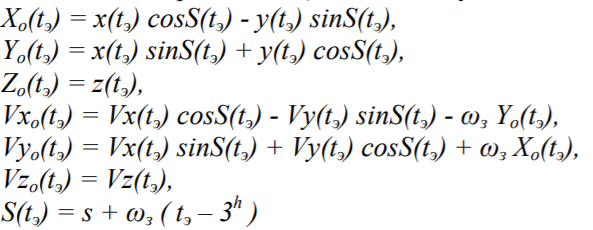
\includegraphics[scale=0.7]{1}}
	\caption{формулы перевода из СК ПЗ-90-02 в абсолютную геоцентрическую СК }
	\label{1}
\end{figure}

Полученные координаты являются начальными условиями для интегрирования. Метод интегрирования Рунге-Кутты 4 порядка, общие формулы на рис.\ref{2}.

\begin{figure}[h!]
	
	\centering{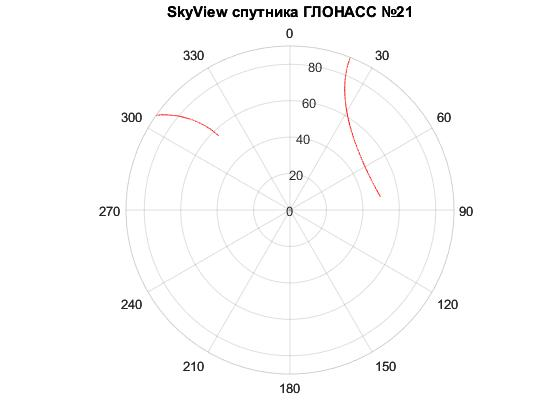
\includegraphics[scale=0.4]{2}}
	\caption{Интегрирование методом Рунге-Кутты 4 порядка }
	\label{2}
\end{figure}


При этом в качестве интегрируемой функции берутся выражения с рис.\ref{3}. Так же в \cite{ICD} указано, что поправки на небесные тела можно учесть однократно, если прибавить их к итоговым вычислениям, воспользовавшись формулой с рис.\ref{4}.В этом случае ошибки возрастут на не более 10\% .


\begin{figure}[h!]
	
	\centering{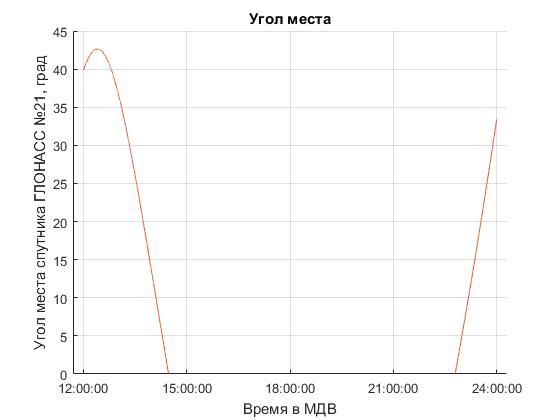
\includegraphics[scale=0.7]{3}}
	\caption{Интегрируемая функция }
	\label{3}
\end{figure}

\begin{figure}[h!]
	
	\centering{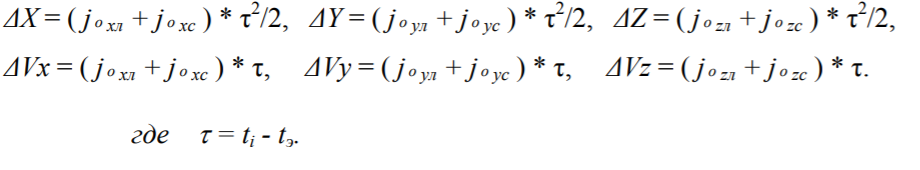
\includegraphics[scale=0.8]{4}}
	\caption{Учет поправок на небесные тела }
	\label{4}
\end{figure}

\section{Практическая реализация}

Для практической реализации на данном этапе использовалась среда Matlab R2019b. Расчетный модуль состоит из одного скрипта, и нескольких функций. 
В главном скрипте выполняется:

1. Задание эфемиридных и временных данных, а так же констант.

2. Пересчет систем координат.

3. Вызов функции расчета временных параметров, вызов функции расчета координат.

4. Моделирование сферы Земли и траекторий НКА по полученным данным.

Всего функций, которые вызываются в данном модуле четыре.
Первая из них, это функция "time". Поскольку функция вызывается лишь единожды, расчеты из нее можно перенести в основной скрипт, но это немного "засорит" программное поле.
Вторая функция "math2" производит расчет координат на интервал времени. Ее так же можно перенести в основной скрипт. В этой функции учтены две ситуации с временным интервалом:
первая- координаты вычисляются на моменты времени больше чем время прихода эфемерид, вторая- координаты вычисляются на время и до, и после времени прихода эфемерид. Если с первым вариантом никаких сложностей не возникает, со вторым связано появление множества "костылей" в программе. Первое что нужно учитывать, это то, что для вычесления координат на более ранее время, нужно интегрировать с шагом -dt. Поскольку вектор каждого навигационного элемента будет инвертирован во времени (т.е $ X=[x_{te}, x_{te-1},...,x_{tstart}]$), его тоже нужно повернуть на 180 градусов. 
На рис.\ref{5} изображена концепция вычисления координат на вес временной интервал. 

 \begin{figure}[h!]
	
	\centering{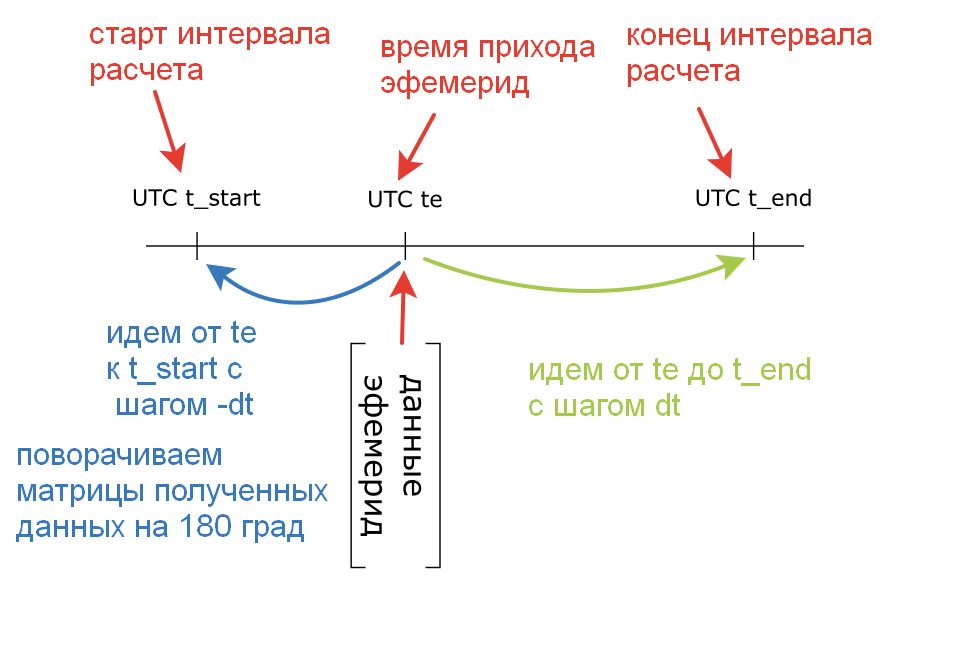
\includegraphics[scale=0.5]{5}}
	\caption{Временные интервалы }
	\label{5}
\end{figure}

Данные для двух временных интервалов вычисляются отдельно, а затем склеиваются. Для вычисления координат для каждого интервала используется функция "RungeKUTT", которая и производит интегрирование начальных значений. Сама интегрируемая функция задана отдельно, и называется "F". Внутри нее происходят вычесления по формулам с рис.\ref{3}. 


После того, как все вычисления выполнены, программа производит моделирование траектории движения НКА в следующих СК:

1. Инерциальная;

2.ПЗ-90;

3.WGS84;

4.Связанная с приемником (SkyVeiw).

Отдельно хочется отметить, что одна из сложностей была в том, что координаты X были с инвертированным знаком, что создавало эффект "перевернутой земли".


\section{Результат работы}
В результате программы были получены следующие графики траекторий движения:

1. В инерциальной СК, рис.\ref{inertz};

2.В СК ПЗ-90, рис.\ref{PZ};

3.В СК WGS84, рис.\ref{WGS};

4.В Связанной с приемником СК (SkyVeiw), рис.\ref{skyv}



\begin{figure}[h!]
	
	\centering{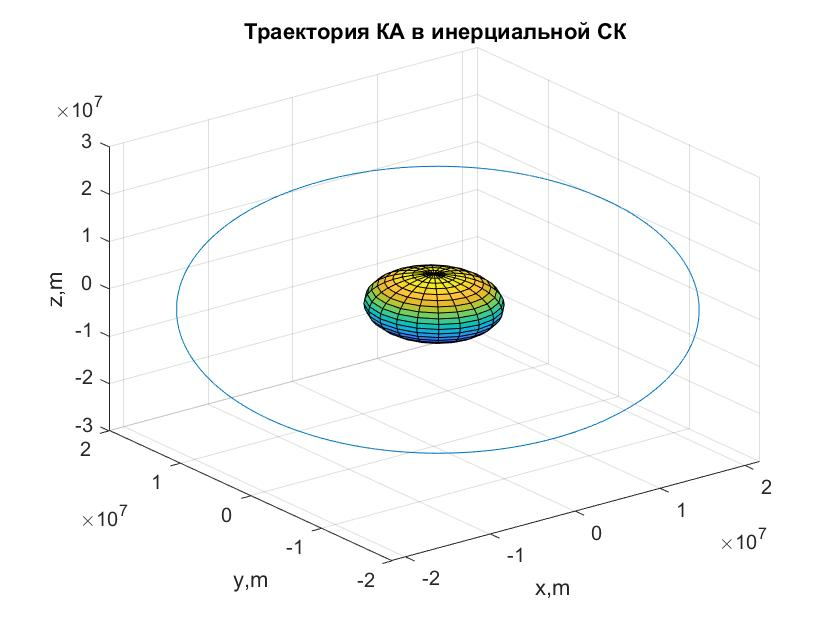
\includegraphics[scale=0.2]{inirtz}}
	\caption{Траектория движения в инерциальной СК  }
	\label{inertz}
\end{figure}

\begin{figure}[h!]
	
	\centering{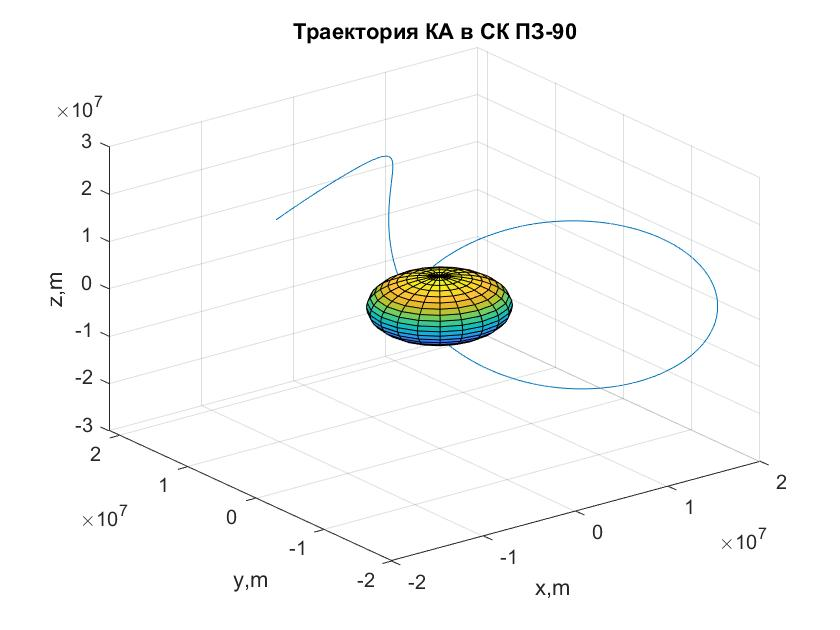
\includegraphics[scale=0.2]{PZ90}}
	\caption{Траектория движения  СК ПЗ-90 }
	\label{PZ}
\end{figure}

\begin{figure}[h!]
	
	\centering{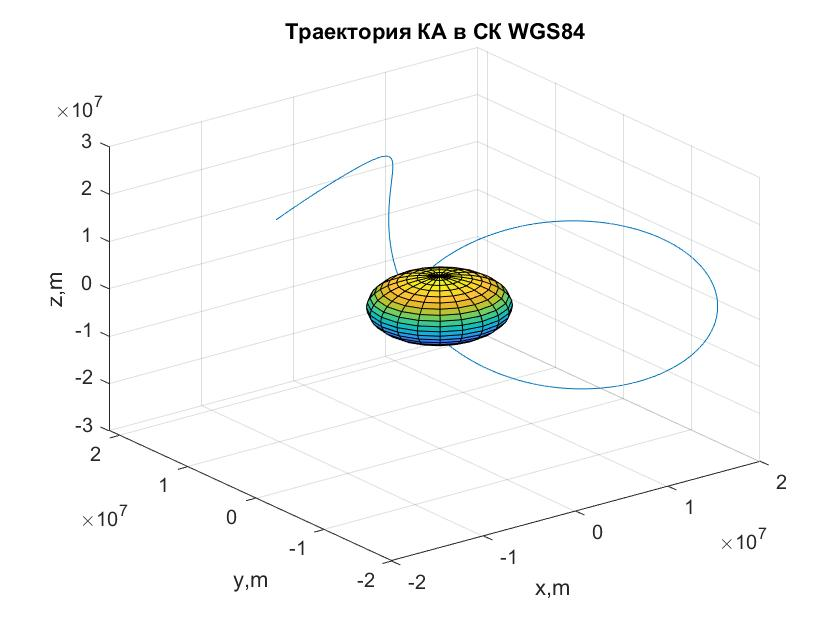
\includegraphics[scale=0.2]{WGS}}
	\caption{Траектория движения в СК WGS84  }
	\label{WGS}
\end{figure}

\begin{figure}[h!]
	
	\centering{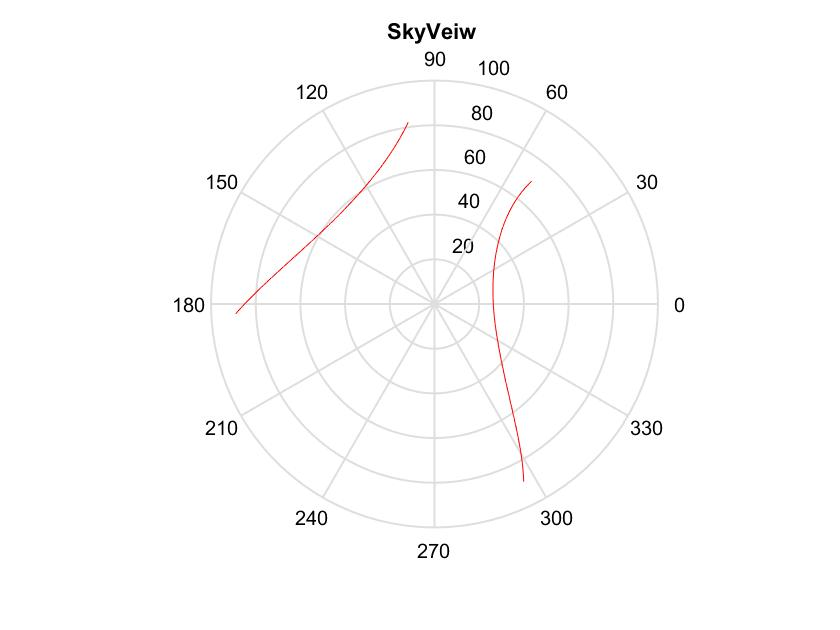
\includegraphics[scale=0.2]{skyv}}
	\caption{Траектория движения в СК связанной с приемником }
	\label{skyv}
\end{figure}


\section{Выводы}

На втором этапе курсового проекта были получены данные о положении НКА на промежуток времени с 12.00 по 24.00 10 февраля 2020 года. Данные эфемерид были взяты с первого этапа курсового проекта. Получены изображения траектории НКА на заданный промежуток времени. По результатам работы на этапе была получена следующая научно-техничекая продукция:

-программа расчета положения НКА;

-графики траекторий НКА на заданный интервал времени;

- Sky View для заданного НКА в заданный промежуток времени.


\newpage
\addcontentsline{toc}{section}{\bibname}
\begin{thebibliography} {7}
	
	\bibitem{ICD} ИКД Глонасс 5.1, 2008
	

\end{thebibliography}

\end{document}
